\section{Introduction}
% \wh{Do you really want to emphasize "large" in the title? To me, large is 100 million. We better leave this to "large-scale challenge" :)}
%introduction to temporal graphs & motivate need for TGL
Many real-world systems such as social networks, transaction networks, and molecular structures can be effectively modeled as graphs, where nodes correspond to entities and edges are relations between entities. Recently, significant advances have been made for machine learning on static graphs, led by the use of \emph{Graph Neural Networks (GNNs)}~\cite{kipfsemi,velivckovic2017graph,chen2019equivalence} and \emph{Graph Transformers}~\cite{rampavsek2022recipe,kreuzer2021rethinking,dwivedi2020generalization}, and accelerated by the availability of public datasets and standardized evaluations protocols, such as the widely adopted \emph{Open Graph Benchmark~(OGB)}~\cite{hu2020open}.  

% \wh{split}

However, most available graph datasets are designed only for {\em static} graphs and lack the fine-grained timestamp information often seen in many real-world networks that evolve over time. Examples include social networks~\cite{pareja2020evolvegcn}, transportation networks~\cite{cini2022scalable}, transaction networks~\cite{shamsi2022chartalist} and trade networks~\cite{poursafaeitowards}.
Such networks are formalized as \emph{Temporal Graphs~(TGs)} where the nodes, edges, and their features change {\em dynamically}. 

A variety of machine learning approaches tailored for learning on TGs have been proposed in recent years, often demonstrating promising performance~\cite{rossi2020temporal,congwe,souza2022provably,luoneighborhood,jin2022neural}. However, Poursafaei \emph{et al.}~\cite{poursafaeitowards} recently revealed an important issue: these TG methods often portray an over-optimistic performance — meaning they appear to perform better than they would in  real-world applications — due to the inherent limitations of commonly used evaluation protocols.

This over-optimism creates serious challenges for researchers. It becomes increasingly difficult to distinguish between the strengths and weaknesses of various methods when their test results suggest similarly high performance. Furthermore, there is a discrepancy between real-world applications of TG methods and the existing evaluation protocols used to assess them. Therefore, there is a pressing need for an open and standardized benchmark that enhance the evaluation process for temporal graph learning, while being aligned with real-world applications.

%introduce our solution

%\wh{Move this up. You can first present TGB, then say how it addresses all the problems. To me, it is best to introduce your method/benchmark within the first third paragraph.}
%\wh{You can say "Here we present TGB..." Otherwise, takes too long to arrive at TGB}
%\wh{This paragraph is very well-written, but too long. Consider splitting it into multiple paragraphs with coherent topic for each para.}


In this work, we present the \emph{Temporal Graph Benchmark~(\name)}, a collection of challenging and diverse benchmark datasets for realistic, reproducible, and robust evaluation for machine learning on temporal graphs. Figure~\ref{Fig:pipeline} shows \name's ML pipeline. Inspired by the success of OGB, \name automates the process of dataset downloading and processing as well as evaluation protocols, and allows the user to easily compare their model performance with other models on the public leaderboard. \name improves the evaluation of temporal graph learning in both \emph{dataset selection} and \emph{evaluation protocol} and covers both edge and node level tasks.

% In this work, we aim to enhance the evaluation of temporal graph learning models in two ways: \emph{dataset selection} and \emph{evaluation protocol}. 

%% Therefore, there is an urgent need to improve the evaluation process for temporal graph learning and ground it in the application. 
% Our work addresses the following two limitations. 

%limited in size, node, edge and duration 
%limited in diversity, focus on social networks
%limited in task, not many available for node level tasks

% \begin{figure*}[t]
%     \begin{center}
%         \centerline{
\includegraphics[width=0.6\textwidth]{figs/dataset_stats.pdf}} %\vspace{-15pt}
%         \caption{ \name consists of a diverse set of datasets (in \textcolor{orange}{orange}) that are one order of magnitude larger than existing datasets in terms of number of nodes, edges and timestamps (in \textcolor{blue}{blue}). The size of the circle is set to be the number of timestamps in log.}
%         %\caption{Dataset statistics. The size of the circles corresponds to (log) number of timestamps. }
%         \label{Fig:data-stats}
%     \end{center}
%     \vskip -0.3in
% \end{figure*}


\begin{wrapfigure}{R}{0.55\textwidth}\vspace{-14pt}
\centering
    
\includegraphics[width=0.55\textwidth]{figs/dataset_stats.pdf}
    \caption{
     \name consists of a diverse set of datasets that are one order of magnitude larger than existing datasets in terms of number of nodes, edges, and timestamps.
    }
\label{fig:data-stats}\vspace{-12pt}
\end{wrapfigure}


%\wh{convincing! great job}
\textbf{Dataset Selection.} 
Contrary to real-world networks that typically contain millions of nodes and tens of millions of edges, existing TG benchmark datasets are notably smaller, falling short by several orders of magnitude~\cite{poursafaeitowards,souza2022provably}. Furthermore, these datasets often have limitations in terms of their domain diversity, with a substantial focus on social and interaction networks~\cite{rossi2020temporal,kumar2019predicting,luoneighborhood}. This lack of diversity can be problematic as network properties, such as network motifs~\cite{milo2002network}, the scale-free property~\cite{broido2019scale}, and the modular structure~\cite{onnela2012taxonomies} vary significantly across different domains. Consequently, it is important to benchmark existing methods across a wide variety of domains for a more comprehensive evaluation.

To address these limitations, \name datasets provide diversity in terms of the number of nodes, edges, timestamps, and network domains. As shown in Figure~\ref{fig:data-stats}, \name datasets are larger in scale and present statistics that were under-explored in prior literature. For instance, \changed{the \token dataset has around 73 million edges} while the \reddit dataset has more than 30 million timestamps. \changed{ Additionally, \name introduces four datasets in the novel \emph{node affinity prediction} task to address the scarcity of large scale datasets for node level tasks in the current literature.}



% {\bf [MB: I think it will be important to add another figure similar to Fig 1 showing the temporal span/number of timestamps of different datasets]} 


% \textbf{Evaluation Protocol.} 
% Temporal graph learning models are often evaluated on binary classification-based link prediction, using one negative edge per positive edge in the test set~\cite{congwe,souza2022provably,luoneighborhood,poursafaeitowards}.


% {\bf [MB: from this description I am not getting if only link prediction or also node classification/regression tasks are proposed]}
% \gr{agreed. Is the contribution on novel evaluation metrics only for the link prediction datasets, or also for node property prediction ones? this is not clear from the previous 2 paragraphs (and lead to confusion wrt the kind of tasks introduced in \name). }

% \textbf{Evaluation Protocol.} 
\changed{Improved Evaluation.}
In \name, we aim to design the evaluation for both edge and node level tasks on temporal graphs based on real applications. Historically, the standard approach for dynamic link prediction evaluation is to treat it as a binary classification task using one negative edge per positive edge in the test set~\cite{congwe,souza2022provably,luoneighborhood,poursafaeitowards}.
This strategy tends to generate negatives that are easy to predict, given the structure and sparsity of real-world networks~\cite{barabasi2013network}, leading to inflated model performance estimations~\cite{poursafaeitowards}. To address this issue,
we propose to treat the task as a ranking problem, contrasting each positive sample against multiple negatives and using Mean Reciprocal Rank~(MRR) as the metric. Moreover, \emph{historical negatives} – past edges absent in the current step – are more difficult to predict correctly than randomly sampled negatives~\cite{poursafaeitowards}. Thus, we sample both historical and random negatives in link prediction evaluations. 

\changed{There is a lack of large scale datasets for node level tasks in temporal graphs as acquiring dynamic node labels remains challenging due to privacy concerns. We plan to include additional datasets for node classification in the future. As a starting point, we present the novel \emph{node affinity prediction} task, which finds its motivation in recommendation systems. The objective is to anticipate the shifts in user preferences for items over time, as expanded in Section~\ref{sub:nodeprop}. In this task, node property is considered as the affinity towards different items at a given time. To assess the effectiveness of methods in addressing this task, we adopt the normalized discounted cumulative gain~(NDCG) metric. This metric serves to determine whether the methods' predictions for class importance adhere to the same ordering as the ground truth.
In Section~\ref{sub:node_exp}, we show that simple heuristics can outperform state-of-the-art TG methods in achieving superior performance for this task.
} 

% we formulate the dynamic node property prediction task which is motivated by applications in churn prediction and recommendation systems where the goal is to predict how the user preference towards items shifts over time~(see Section~\ref{sub:nodeprop}). 
% Here, node property is considered as the affinity towards different items at a given time. For this task, we select the normalized discounted cumulative gain~(NDCG) metric to evaluate if methods output node labels that respect the same ordering of classes as the groundtruth. In Section~\ref{sub:node_exp}, we show that simple heuristics can outperform state-of-the-art TG methods in this task.
% Secondly, for the dynamic node property prediction task, we select the normalized discounted cumulative gain~(NDCG) metric to evaluate if methods output node labels that respect the same ordering of classes as the groundtruth. Finally, we include simple baselines for both tasks, revealing that heuristics can sometimes match or even exceed the performance of more complex models. 

Overall, our proposed Temporal Graph Benchmark has the following contributions: 
\begin{itemize}
    \item \textbf{Large and diverse datasets.} \name includes datasets coming from a diverse range of domains and spanning both node and edge-level tasks. \changed{We contributed seven novel datasets which are orders of magnitude larger than existing ones in terms of number of edges, nodes and timestamps.}
    % Seven of the datasets are novel and curated for this benchmark.
    
    %We also included three datasets for node level task to address the sparsity of datasets with dynamic node labels in the literature. 
    % \ah{rephrase here}
    % Empirically, we found that model performance and ranking can vary significantly across datasets. 

    \item \textbf{Improved evaluation.} We propose an improved and standardized evaluation pipeline motivated by real-world applications. For dynamic link property prediction, we sample multiple negative samples per positive edge and ensure a mix of both historical and random negative samples, while using the \emph{MRR} metric. \changed{For the node affinity prediction task, we use the \emph{NDCG} metric to evaluate the relative importance of classes within the top ranking ones.}
    
    % we use the \emph{NDCG} metric to evaluate the relative ordering of node labels within the top ranked classes.

    % \item \textbf{Improved evaluation for link prediction.} \name improves and standardizes the evaluation procedure for link prediction on temporal graphs. Specifically, we propose to evaluate against more negative samples per positive edge and ensure a mix of both historical and random negative samples in evaluation. We also propose to use the \emph{MRR} metric commonly used in knowledge graph literature to examine the rank of the true edge amongst multiple negatives~\cite{wang2022interht,hu2020open}. The \name evaluation protocol leads to clear performance distinctions among state-of-the-art (SOTA) TG methods, while also leaving room for improvement for future methods. 
    
    % \item \textbf{Novel dynamic node property prediction task.} \name includes the novel \emph{dynamic node property prediction} task as an extension of the node property prediction task on static graphs to TG. Here, the goal is to predict the property of a given node at a future time. Example applications include churn prediction and recommendation systems where the prediction of user preference towards some items is highly important. Empirically, we observe that current SOTA methods have little performance advantage over simple heuristics such as moving average and persistence forecast in this task. \todo{ER: If I were a reviewer, this would be confusing because you are claiming that you are the first one to introduce dynamic node classification} \wh{Has temporal graph learning community already explored this task type? If so, we should emphasize it. If not, we should tone down.}
    
    % \item \textbf{Novel node-level tasks:} \name proposes a novel node-level task for temporal graphs, the node property prediction task which aims to predict the distribution of which nodes a given node will interact with in the future. \mf{is this correct? This reads like a link-prediction task.} This task has strong practical implications in recommendation systems and churn prediction. \todo[inline]{ER: We need to be careful here, because it reads a bit as we're the first to propose node level task for temporal graphs, which is obviously not the case. What is exactly our contribution here? To reframe a recommender system question as a node classification task?} \gr{agreed. We should likely come up with another name than "Node property prediction" more clearly referring to the task we are considering here. }

    % performance of different models are now distinct from each other.
    %Moreover, datasets with a higher ratio of test edges which are unseen during training are more challenging for all methods.
    \item \textbf{Empirical findings.} We show that for the dynamic link property prediction task, model performances can vary drastically across datasets. \changed{For example, the best performing model on \wikipedia encounters a 40\% test MRR drop on \review and the \emph{surprise index} of a dataset affects model performance.} On the \changed{node affinity prediction task}, we find that simple heuristics can often outperform state-of-the-art TG methods, thus leaving ample room for development of future methods targeting this task. 
    
    % We compare a large number of methods on our datasets. TGN seems to be the best performing model across the board, since it can be used in both link property prediction and node property prediction, while also scaling to large datasets. Interestingly, we however find that simple heuristics are often outperforming or matching TGN and other ML methods on dynamic node property prediction datasets, leaving ample room for development of methods aimed at this specific task. 
    % \ah{add more findings here}

    \item \textbf{Public leaderboard and reproducible results.} Following the good practice of OGB, \name also provides an automated and reproducible pipeline for both link and node property prediction tasks. Researchers can submit and compare method performance on the \name leaderboard. 
    %\wh{what is node affinity prediction? I think it's just temporal node/link property prediction.} \wh{These automated pipeline and leaderboard is too similar to OGB. Better to give credit to OGB by saying "inspired by the design of OGB...".}
\end{itemize}

\textbf{Reproducibility:} \name code, datasets, leaderboards and details are on the \href{https://tgb.complexdatalab.com/}{\name website}. The code is also publicly available on \href{https://github.com/shenyangHuang/TGB}{GitHub} with documentations seen \href{https://docs.tgb.complexdatalab.com/}{here}.


% \wh{Add experiments/findings as your contribution as well.}
% \todo{ER: Especially the lack of methods that work well on dynamic node prediction, probably because the focus so far on link prediction (caused by the lack of node prediction datasets)}
% \wh{Cite knowledge graph work on filtered MRR. It's very common there.}
    %We also conduct extensive comparison with the simple baseline Edgebank and show that it can achiev
    %We also show that on some datasets, a simple heuristics Edgebank can perform competitively against SOTA methods. 
        
    % \wh{To me, this is okay novelty. Evaluating against all negatives is very commonly done in knowledge graph completion and recommender system literature. This is just not adopted by the temporal link prediction community, and we are resolving that. }
    % \ah{I agree, I also added more empirical benefits of the novel evaluation to the discussion. }
 % or interactive pattern of a given node towards a set of specified nodes in the graph over a future period. This task has important applications in churn prediction and recommendation systems. We observe that current SOTA methods are less performant than simple heuristics such as persistant forecast and moving average in this task and there is significant room for improvement in this task. 
    % \ah{updated to distinguish from node classification task}


\begin{figure*}[t]
    \begin{center}
        \centerline{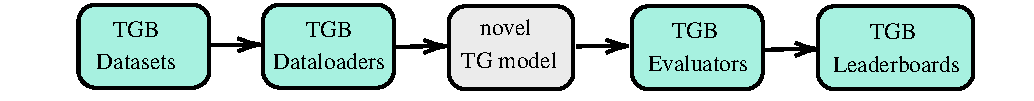
\includegraphics[width=\textwidth]{figs/tgb_pipeline.pdf}} %\vspace{-15pt}
        \caption{\textbf{Overview of the Temporal Graph Benchmark~(\name) pipeline:} \textbf{(a)} \name includes large-scale and realistic datasets from five different domains with both dynamic link prediction and node property prediction tasks. \textbf{(b)} \name automatically downloads datasets and processes them into \texttt{numpy}, PyTorch and PyG compatible \texttt{TemporalData} formats. \textbf{(c)} Novel TG models can be easily evaluated on \name datasets via reproducible and realistic evaluation protocols. \textbf{(d)} \name provides public and online leaderboards to track recent developments in temporal graph learning domain. The code is publicly available as a Python library. }
        \label{Fig:pipeline}
    \end{center}
    \vskip -0.4in
\end{figure*}
% \todo[inline]{ER: Can we make this diagram more similar in colors and naming to the OGB ones. Colors don't look great}

% \wh{Beyond the datasets, one important insight that we should emphasize is the extensive performance comparison against the simple baseline methods. That's one of the most important contributions of TGB. In the intro, we may expand a bit about what simple baselines are, and how they perform against SoTA temporal GNN models. And discuss some insight/future work based on baseline experiments.}

% Previous research experiments often lack comparisons to simple baselines or heuristics, which we show can sometimes achieve surprisingly competitive performance to more complex models.% The commonly used AU-ROC metric is an unsuitable metric when there is more than one negative sample per positive one during evaluation. \wh{Why ROC-AUC cannot handle multiple negatives per positive. I think it can, but just does not reflect the topK nature.}
% \wh{Intro and the entire project reads very similar to OGB. Good to point out the similarity and differences to OGB. The difference part is the most important.}


% Lastly, in the context of temporal graph learning, due to the scarcity of the datasets with dynamic node labels, node-level tasks have received significantly less attention compared to edge-level tasks. \name includes three datasets for the dynamic node property prediction task in different sizes.

% limited negative samples
% AUROC is not a good metric
% using ndcg for dynamic node label 
% \wh{"Next" sounds weird transition} Next % Thus, during evaluation, there should be significantly more negative examples than positive ones.
%it is important to incorporate these historical negatives in addition to random negatives when evaluating for link prediction. 
%As link prediction is the most common task in literature, we focus on our discussion on link prediction evaluation here. 











% Motivations for this work:
% \begin{itemize}
%     \item current benchmark datasets are small and lacks domain diversity
%     \item current link prediction evaluation only samples one negative per positive, highly unrealistic thus resulting in all methods achieving extremely optimistic performance, difficulty to tell the performance difference. 
%     \item lack of node level datasets
%     \item lack of standardized, open and reproducible evaluation pipeline with public leaderboard

%     % \item current temporal graph benchmarks are small in scale, usually limited to < 2 million edges across all timestamps
%     % \item current evaluation procedure is disjoint from real applications 
%     % \item Many methods achieve extremely high performance on existing benchmarks and difficult to distinguish between methods
% \end{itemize}

% goal: facilitate scalable, applicable, robust  and reproducible temporal graph research


% Contributions:
% \begin{itemize}
%     \item new datasets to address previous limitation, limited size, domain diversity, lack of edge / node feature
%     \item simple baselines work surprisingly well, and need future research to improve upon them
%     \item new evaluation procedure with more negative samples and unifying different idea for sampling, new metric, f1@k, and filtered mrr? 
%     \item new task, node proprety prediction, for learning the evolution of node behaviors in temporal graph for realistic applications
%     \item online and accessible leaderboard, dataset downloading processing, available pip install 
% \end{itemize}






% We present the Temporal Graph Benchmark~(\name): a collection of challenging and diverse benchmark datasets for realistic, reproducible and robust evaluation for temporal graph research.\name is motivated by three major limitations of current evaluation setups: 1). \emph{limited graph sizes}: almost all benchmark datasets are small with less than 2 million edges, 2). \emph{too few negative samples}: current evaluation for link prediction only samples one negative edge per positive edge, this is highly unrealistic and 3). \emph{lacking features}: all benchmark datasets contains no edge features outside of a few with edge weights. In this work, we addresses these limitations by adding new datasets ranging from 4 million to 67 million, orders of magnitude larger than existing ones. Then we improves the evaluation for link prediction by sampling hundreds of negative edges per single positive edge. Lastly, we include additional edge and node features where possible to enrich the datasets. 